% Oliver Kullmann, 15.5.2016 (Swansea)
% The bibtex-entry of this paper is \cite{AbbasizanjaniKullmann2016MU2}.

% Switching between report- and journal-version: uncomment the appropriate
% block of definitions of \Schrift, \Liste.

\documentclass{article}

\usepackage{a4}

\input Latex_macros/Definitionen.tex

\usepackage{enumerate}
\usepackage[active]{srcltx}
\usepackage[all]{xy}
%\usepackage{graphicx}



\newcommand{\Schrift}{report}
\newcommand{\Liste}{minimal unsatisfiability \sep deficiency \sep finiteness conjecture}
%\newcommand{\Schrift}{article}
%\newcommand{\Liste}{}

\providecommand{\keywords}[1]{\textbf{\textit{Keywords}} #1}
\providecommand{\sep}{, }

\nc{\tsubres}{\xrightarrow{\text{sfsR}}}
\nc{\tsubresk}[1]{\xrightarrow{\text{sfsR}}_{\!#1}}
\DMO{\saturate}{S}


\begin{document}

\title{Understanding minimal unsatisfiability for two more clauses than variables}

\author{
  \href{XXX}{Hoda Abbasizanjani}\\
  Computer Science Department\\
  Swansea University\\
  Swansea, SA2 8PP, UK
  \and
  \href{http://cs.swan.ac.uk/~csoliver}{Oliver Kullmann}\\
  Computer Science Department\\
  Swansea University\\
  Swansea, SA2 8PP, UK
}

\maketitle

\begin{abstract}
  properly understanding
\end{abstract}

\keywords{\Liste}

\tableofcontents


\setcounter{section}{-1}
\section{TODOS}
\label{sec:todos}


\subsection{Outline}
\label{sec:Outline}

\begin{enumerate}
\item The minimal program is to present short and intuitive proofs for the characterisations of $\Musati{\delta=1}$ and $\Musatnsi{\delta=2}$.

  The appropriate venue for publication would be \href{http://www.sciencedirect.com/science/journal/00200190}{IPL}.
\item One could also go for a ``fuller understanding'':
  \begin{enumerate}
  \item Covering to some degree (all of) $\Musati{\delta=2}$.
    \begin{enumerate}
    \item Describing the subclasses $\Uclashi{\delta=2}$ and $\Smusati{\delta=2}$.
    \item Determining the clause-irreducible elements of $\Musati{\delta=2}$, extending \cite[Lemma 41]{KullmannZhao2016UHitSAT}. A relevant question here is how far \cite[Lemma 36]{KullmannZhao2016UHitSAT} can be generalised; especially whether for $F \in \Musati{\delta=2}$ holds, that clause-irreducibility implies non-singularity?!
    \end{enumerate}
  \item Describing parameters like minimum var-degree, number of (1-)singular variables, singularity index, number of full clauses, number of full variables, unit-clauses. See \cite[Section 5]{KullmannZhao2016UHit}.
  \item Determining hardness and asymmetric width, and moreover precise determination of resolution- and tree-resolution-complexity.
  \item Determining the hermitian rank and related measures.
  \item Counting the number of non-isomorphic elements for a given number of clauses.
  \end{enumerate}
\item A proper new Theorem would be, if one could give a model for $\Musati{\delta=2}$ (combining somehow the tree-model for $\Musati{\delta=1}$ and the circle-model for $\Musatnsi{\delta=2}$).
\item For the ``full underlying report'' (this \Schrift), we don't restrict ourselves, and only later will we see how to publish it (perhaps just one short paper, perhaps several short papers, perhaps one longer paper, ...).
\end{enumerate}


\subsection{Proposed tasks for HA}

\begin{enumerate}
\item Collect and expand the literature (here, with details):
  \begin{enumerate}
  \item Deficiency $1$: see \cite{KullmannZhao2010Extremal} for an overview. (done)
  \item Deficiency $2$: \cite{KleineBuening2000SubclassesMU} is the starting point. (done)
  \end{enumerate}
\item Add references appropriately. (done)
\item Understand the known proofs for characterisation/construction of $\Musati{\delta=1}$ (see \cite{KullmannZhao2010Extremal} for an overview). (done)
\item Determine all the measures for the $\Dt{n}$.
\item Understand the basic tools (see \cite{KullmannZhao2010Extremal}): (done)
  \begin{enumerate}
  \item every element of $\Musati{\delta=2}$ has a variable occurring at most $4$ times;
  \item saturation;
  \item splitting on a variable with minimum degree, which must occur here twice positively and twice negatively, yields in both cases an element of $\Musati{\delta=1}$.
  \end{enumerate}
\item Which elements of $\Musati{\delta=1}$ have full clauses?
\item Investigate the special elements of $\Musati{\delta=1}$ obtained via splitting, with two characterisations: Horn clause-sets, and the underlying tree $T$ has Horton-Strahler number $\hts(T) \le 1$. (done)
\item Understand how $\Musati{\delta=2}$ is obtained from $\Musatnsi{\delta=2}$ via singular expansion. (done)
  \begin{enumerate}
  \item And especially understand how $\Smusati{\delta=2}$ is obtained from $\Smusatnsi{\delta=2}$ via saturated singular expansion.
  \item Create catalogues of elements of $\Musati{\delta=2}$ and its subclasses for small number of clauses.
  \item Determine all the measures for the elements of the catalogue.
  \end{enumerate}
\item For a non-trivial binary tree $T$ and $F(T) \in \Uclashi{\delta=1}$, is the number of 1-singular variables in $F(T)$ equal $2^{\hts(T)-1}$ ?
\item Is every element of $\Musati{\delta=2}$ obtained (modulo renaming) from some $\Dt{n}$, by expanding every clause via variable-disjoint elements from $\Musati{\delta=1}$ ?
  \begin{enumerate}
  \item So we start with $\Musatnsi{\delta=2}$, and use the expansion process, which takes an $F \in \Musati{\delta=2}$ and a $C \in F$, and creates a clause-factorisation $F' := (F,C) \cor G$ for some $G \in \Musati{\delta=1}$ according to \cite[Definition 27]{KullmannZhao2016UHitSAT} with $\var(F) \cap \var(G)$, where then $F' \in \Musati{\delta=2}$ holds.
  \item It is superfluous here to consider any $C \in F$ which has already been created by a previous clause-factorisation.
  \item One can also ask the same question for $\Smusati{\delta=2}$, where here then $G \in \Smusati{\delta=1}$ is considered.
  \item A counter-example already for $c=5$ should be given by the example for the singular extensions of $\Dt{2}$ as given in \cite{KullmannZhao2014UHit}.
  \end{enumerate}
  \item For an arbitrary $F \in \Uclashi{\delta=2}$, is it possible to get $F' \not \in \Uclashi{\delta=2}$ by making a saturation extension of $F$?
  \item Determining the number of isomorphic types of clause-sets obtained from $\Dt{n}$ by the following methods:
  \begin{enumerate}
  \item singular extension of $\Dt{n}$.
  \item saturated extension of $\Dt{n}$.
  \item the extension of unsatisfiable hitting clause-sets of $\Dt{2}$ (that is $\Dt{2}, \Dt{3}$).
  \end{enumerate}
\end{enumerate}


\subsection{Proposed tasks for OK}

\begin{enumerate}
\item Currently no specific tasks.
\end{enumerate}




\section{Introduction}
\label{sec:intro}

%%%%%%%%%%%%%%%%%%%%%%%%%%%%%%%%%%%%%%%%%%%%%%%
\section{Preliminaries}
\label{cha:Preliminaries}

\begin{defi}\label{def:dpredc}
By \cite{KullmannZhao2010Extremal}, the \textbf{DP-reduction} is the process of removing a variable $v \in \var(F)$ by taking all clauses having $v$ and replacing them by their resolvents that is:
\begin{displaymath}
\bmm{\dpi{v}(F)} := \set{C \in F : v \notin \var(C)} \cup \set{C \res D : C, D \in F \und C \cap \ol{D} = \set{v}} \in \Cls
\end{displaymath}
\end{defi}
Remarks:
  \begin{enumerate}
  \item If two clauses $C,D \in F$ have more than one clashes, by performing the DP-reduction on one of clashing variables both clauses are removed and we get nothing .
   \end{enumerate}
   
\begin{defi}\label{def:mu}
A clause-set $F \in \Usat$ is \textbf{minimally unsatisfiable} if by removing any arbitrary clause $C \in F$, the clause-set $F \sm \set{C}$ becomes satisfiable. The set of all minimally unsatisfiable clause-sets is $\bmm{\Musat} \in \Usat$.
\end{defi}
Remarks:
  \begin{enumerate}
  \item The complexity of the problem $\Musat \in \Usat$ is $D^P$-complete (by Theorem 11.1.1 in \cite{Kullmann2007HandbuchMU}).
  \item All full clause-sets $ A_n$ are in $\Musati{}$.
  \end{enumerate}

\begin{defi}\label{def:deficiency}
The \textbf{deficiency} for a clause-set $F \in \Cls$ is defined as the difference between the number of clauses and the number of variables and denoted by $\bmm{\delta} \in \ZZ: \delta(F)= c(F) - n(F)$.
\end{defi}
Remarks:
  \begin{enumerate}
  \item In this report, the minimally unsatisfiable clause-sets with deficiency $k \in \ZZ$ are denoted by $\Musati{\delta=k}$.
  \item The complexity of the problem $\Musati{\delta=k}$ with fixed $k$ is $P$ (by Theorem 11.2.1 in \cite{Kullmann2007HandbuchMU}).
  \item All $F \in \Musati{\delta=k}$ have $k \ge 1$ (by Theorem 8 in \cite{DDK98}).
  \end{enumerate}

\begin{defi}\label{def:degree}
For a clause-set $F \in \Cls$ the \textbf{literal degree} for a literal $x \in \lit(F)$ is the number of the literal occurrence and denoted by $\bmm{\ldeg_F(x)} \in \NNZ$. The \textbf{variable degree} for a variable $v \in \var(F)$ is defined as $\bmm{\vdeg_F(v)} := \ldeg_F(v) + \ldeg_F(-v) \in \NNZ$. Also, the \textbf{minimum variable degree} (or min-var-deg) is defined as the minimum of variable degree for all variables in $F$ and denoted by $\bmm{\minvdeg(F)} \in \NN$.
\end{defi}
Remarks:
  \begin{enumerate}
  \item It is obvious that $\vdeg_F(v) \le 2 \delta(F)$ and thus for $n(F) >0$, $\minvdeg(F) \le 2 \delta(F)$. A sharper upper bound for $\minvdeg(F)$ is given in Theorem 9.10 of \cite{KullmannZhao2010Extremal}.
  \item All full clauses $A_n$ have deficiency $2^n - n$ and if $n \ge 1$, then  $\minvdeg(A_n) =2^n$.
  \item In \cite{KullmannZhao2010Extremal}, the problem of finding the min-var-deg for minimally unsatisfiable clause-sets with fixed deficiency is denoted by $\minnonmer(k) $ (that is $\minnonmer(k)  :=  \minvdeg(\Musati{\delta=k}) \in \NN$) and an improved upper bound/ lower bound for $\minnonmer(k) $ is given.
    \end{enumerate}
    
\begin{defi}\label{def:singvar}
By \cite{KullmannZhao2012ConfluenceJ}, for a non-pure variable $v \in \var(F)$ if $\min(\ldeg_F(v) ,\ldeg_F(-v))=1$, then it is called a \textbf{singular variable}. If a clause-set $F$ does not have any singular variable, it is called \textbf{nonsingular}. An \textbf{m-singular variable} is a singular variable with $\vdeg_F(v)=m+1$, $m \in \NN$.
\end{defi}
Remarks:
  \begin{enumerate}
  \item The set of nonsingular minimally unsatisfiable clause-sets $F \in \Musat$ is denoted by $\bmm{\Musat'} \in \Musat$. Thus, if $F \in \Musat'$, then all variables in $F$ are occurred at least twice positively and at least twice negatively.
  \item A \textbf{non-1-singular variable} is a variable which $m$-singular for some $m \ge 2$.
   \end{enumerate}
 
\begin{defi}\label{def:splitting}
For $F \in \Cls$, consider a variable $v \in \var(F)$. \textbf{Splitting} of $F$ on $v$ is the process of obtaining two clause-set $F_0,F_1$ such that  $F_0:=\pao v0 * F$ and $F_1:=\pao v1 * F$.
\end{defi}
Remarks:
  \begin{enumerate}
  \item For $F \in\Musati{\delta=k}$, splitting may lead to produce two minimally unsatisfiable clause-sets $F_0,F_1$ but generally one can not speak of minimally unsatisfiability unless more information is provided. 
  \item For $F \in\Musatnsi{\delta=k}$ if after splitting on a variable $v \in \var(F)$ the clause-sets $F_0,F_1$ are minimally unsatisfiable with deficiency $k_0, k_1$, then we have $k_0, k_1 < k$ (by Theorem 2 in \cite{KleineBuening2000SubclassesMU}).
  \end{enumerate}
%------------------------------------------------------------------------------------------------------------
\begin{defi}\label{def:smu}
A clause set $F \in \Cls$ is called \textbf{saturated} minimally unsatisfiable iff $F \in \Musat $ and by replacing any $C \in F$ by any super-clause $C' \supset C$, the result clause-set is satisfiable. The set of all saturated minimally unsatisfiable clause-sets is denoted $\bmm{\Smusat} \subset \Musat$.
\end{defi}
Remarks:
  \begin{enumerate}
  \item The set of all nonsingular saturated minimally unsatisfiable clause-sets is $\bmm{\Smusatns} \subset \Smusat$.
  \item For all clause-sets $F \in \Cls$, if $F \in \Uclash$ then $ F \in \Smusat$ ,i.e. $\Uclash \subset \Smusat$ (by Lemma 2 in \cite{KullmannZhao2012ConfluenceJ}). 
  \item For every $F \in \Musat$ there is a saturation $F' \in \Smusat$. A saturated clause-set  $F'$ for $F$ is obtained using an operation defined in Definition \ref{def:smu-opr}.
  \end{enumerate}

\begin{defi}\label{def:smu-opr}
\cite{KullmannZhao2012ConfluenceJ} For every $F \in \Musat$ a saturation $F' \in \Smusat$ is obtained by iterated application of the operation $\saturate(F,C,x)$ as follows where $C \in F$, $x \in \lit(F)$ and $\var(x) \not \in \var(C)$:
  \begin{displaymath}
    \bmm{\saturate(F,C,x)} := (F \sm \set{C}) \cup (C \addcup \set{x}) \in \Cls
  \end{displaymath}
If in iteration $m$ there is no literal in $F$ fulfilling the conditions $\var(x) \not \in \var(C)$ for all clauses of $F$ and $F_m \in \Usat$, then $F' =F_m=\saturate(F_{m-1},C_{m-1},x_{m-1}) \in \Smusat$. 
\end{defi}
Remarks:
  \begin{enumerate}
  \item If $F' \in \Smusat$ is a saturation for $F \in \Musat$, then we have $n(F')=n(F)$, $c(F')=c(F)$ and $\delta(F')=\delta(F)$.
  \item If $C \in F$ and $\var(C) = \var(F)$ (full clause), then no literal can be added to $C$ to make $F$ saturated. Also, all full clauses $A_n$ are in $\Smusat$.
  \item By \cite{Ku99dK}, we have $ \Smusati{\delta=k} \subset \Musati{\delta=k} \subset \Lean_{\delta=k} \subset \Usat_{\delta=k} \cup \set{\top} $ which are poly-time decidable.
  \end{enumerate} 
  
\begin{examp}\label{exp:smu-exp}
 For $F = \set{\set{a,b},\set{\ol{a}},\set{\ol{b}}} \in \Musat \sm \Smusat$ using the Definition \ref{def:smu-opr} we can have $F'=\set{\set{a,b},\set{\ol{a},b},\set{\ol{b}}} \in \Smusat$ or $F'=\set{\set{a,b},\set{\ol{a}},\set{a,\ol{b}}} \in \Smusat$.
\end{examp}

\begin{lem}\label{lem:smu-mu}
By \cite{KullmannZhao2010Extremal}  $F' \in \Smusat$ iff for all $v \in \var(F)$, $\langle v \ra 1 \rangle*F \in \Musat$.
\end{lem}

\begin{lem}\label{lem:smu-app}
By \cite{KullmannZhao2010Extremal}, consider a clause-set $F \in \Smusat$. If $F$ is a full clause-set and also it is the saturation of some $F' \in \Musat$, then $F' = F$. Otherwise, if $F$ is not a full clause-set then there exist some some $F' \in \Musat$ with $F' \not= F$ such that $F$ is a saturation of $F'$.
\end{lem}

\begin{quest}\label{que:smu-elim}
For a clause-set $F \in \Smusat$ if $F'$ is obtained by eliminating a literal occurrences in $F$, is $F'$ still minimally unsatisfiable? (that is for $C \in F$, $x \in C$, whether $F' := (F \sm \set{C}) \addcup \set{C \sm \set{x}}$ is in $\Musat$ ?)
\end{quest}
%---------------------------------------------------------------------------------------------------------------------
\begin{defi}\label{def:singularDP}
Consider DP-reduction in Definition \ref{def:dpredc}. If a DP-reduction is performed for a singular variable, then it is called a \textbf{singular DP-reduction} and the set of all nonsingular clause-sets obtainable from $F$ by singular DP-reduction denoted by $\bmm{sDP(F)}$. 
\end{defi}
Remarks:
  \begin{enumerate}
  \item Base on Lemma 5.3 in \cite{KullmannZhao2010Extremal}, if a clause-set $F$ is minimally unsatisfiable then after performing the singular DP-reduction, the result clause-set $F'$ is also minimally unsatisfiable. This is also true when $F$ is in $\Smusat$ or $\Uclash$.   Further more, the singular DP-reduction does not change the deficiency of $F$ since $c(F)$ and $n(F)$ both decreased by one (an overview of DP-reduction for minimally unsatisfiable clause-sets is presented in \cite{KullmannZhao2012ConfluenceJ}).
  \item If $F \not \in \Musat$, then after singular DP-reduction the result is also not minimally unsatisfiable.
  \end{enumerate}
  
\begin{lem}\label{lem:sDP-infl}
For a clause-set $F \in \Musati{\delta=k}$:
  \begin{enumerate}
  \item If $k=1$, then an iterated application of singular DP-reduction leads to $\set{\bot}$ (that is $sDP(F)=\set{\bot}$).
  \item If $k \ge 2$, then an iterated application of singular DP-reduction leads to a clause-set in $\Musatnsi{\delta=k}$ (by Lemma 1 in \cite{KleineBuening2000SubclassesMU}).
  \end{enumerate}
\end{lem} 

\begin{lem}\label{lem:sDP-size}
By \cite{KullmannZhao2012ConfluenceJ}, for $S \in \Smusat$ we have $\abs{\sdp(F)} = 1$.
\end{lem} 

\begin{defi}\label{def:singularextn}
By \cite{KullmannZhao2010Extremal} for a clause-set $F \in\Cls$ and a variable $x \not \in \var(F)$, a \textbf{singular extension} is defined as the reverse direction of a singular DP-reduction. Thus, for obtaining a \textbf{singular m-extension} $F' $of $F$ with $x$, first we choose $m$ different clauses $D_i:D_1, \dots, D_m \in F$. Then, we consider a clause  $C: C \sse \bca_{i=1}^m D_i$. In the next step, for every $D_i$ we consider a clause $D_i':(D_i \sm C) \sse D_i' \sse D_i$. Finally, we obtain $C' := C \addcup \set{x}$, and $D_i'' := D_i' \addcup \set{\ol{x}}$ for $i \in \tb 1m$. Then, we have:
  \begin{displaymath}
    F' := (F \sm \set{D_1,\dots,D_m}) \addcup \set{C', D_1'',\dots,D_m''}.
  \end{displaymath}
\end{defi}
Remarks:
  \begin{enumerate}
  \item Consider an $m$-extension $F'$ of $F$. Then, $F \in \Musat \iff F' \in \Musat$ (by Lemma 5.9 in \cite{KullmannZhao2010Extremal}).
  \item The singular m-extension of $F$ does not change the deficiency of $F$. But, number of clauses (and variables) is increased by one.
  \end{enumerate}
  
\begin{defi}\label{def:unit-ext}
By \cite{KullmannZhao2010Extremal} for a clause-set $F \in \Cls$, a \textbf{full singular unit-extension} $F' \in \Cls$ is obtained as follows: First, consider a literal $x:\var(x) \notin \var(F)$. Then, $F' := \set{\set{x}} \addcup \set{C \addcup \set{\ol{x}} : C \in F}$. Thus, $F' $ has a unit clause $\set{x}$ and all clauses of $F$ with literal $\ol{x}$ added to them.
\end{defi}
Remarks:
  \begin{enumerate}
  \item Consider $F'$ as the full singular unit-extension of $F$, if $F \in \Musati{\delta=k} $ the  $F' \in \Musati{\delta=k} $. This is also true about $F \in \Smusati{\delta=k}$. (by Lemma 5.17 in \cite{KullmannZhao2010Extremal}).
  \end{enumerate}
  
  \begin{defi}\label{def:sres}
The \textbf{subsumption resolution} is a reduction of a clause-set $F \in \Cls$ to $F' \in \Cls$ by removing a literal $x : \var{x} \in \var{F}$ from a clause $C:C \in F$ when there is a clause $D \in F: \ol x \in D$ and also $D \sm \set{\ol x} \sse C$. This means that the resolution of $C,D$ subsumes $C$. Note that $D$ is still in $F'$.
\end{defi}

\begin{defi}\label{def:fsr}
\cite{KullmannZhao2010Extremal} The \textbf{strict full subsumption resolution} is the reduction of $F \in \Cls$ to $F'\in \Cls$ as follows and denoted by $\bmm{F \tsubres F'}$. To obtain $F'$, consider a clause $R \in F'$ (the resolvent) and a literal $x \in \var(F'):\var(x) \notin R$ ($x, \ol{x}$ the resolution literals). Then if $C := R \addcup \set{x}$ and $D := R \addcup \set{\ol{x}}$ (the parent clauses), then we have $F = (F' \sm \set{R}) \addcup \set{C,D}$.

$F \tsubresk{k} F'$ for $k \in \NNZ$ shows the application of exactly $k$ steps of strict full subsumption resolution. 
\end{defi}
   
\begin{defi}\label{def:fse}
Based on \cite{KullmannZhao2010Extremal} the \textbf{strict full subsumption extension} in the reverse direction of the strict full subsumption resolution. Thus by considering the parameters in Definition \ref{def:fsr} for $F, F'$ and $F \tsubres F'$, the clause $R$ is expanded to $C = R \addcup \set{x}$, $D = R \addcup \set{\ol{x}}$ and we say $F$ is obtained from $F'$ by strict full subsumption extension.
\end{defi}
Remarks:
  \begin{enumerate}
  \item If  $F \tsubres F'$ and $F \in \Musat $ then $ F' \in \Musat$ and also if $F \in \Smusat$ we have $ F' \in \Smusat$ while if $ F' \in \Smusat$ then $F \in \Musat $ ( by Lemma 6.5 in \cite{KullmannZhao2010Extremal}). 
  \item Note that for the full subsumption resolution/ extension for the resolution variable $v$, if $v$ is occurred in other clauses then it is called \textbf{strict} but if the variable is vanished it is called \textbf{non-strict}.
  \end{enumerate}
  
\begin{lem}\label{lem:mu-refu-tree}
Based on \cite{KleineBuening2000SubclassesMU} if $F \in \Musati{\delta=k}$ then an iterated application of singular DP-reduction and the splitting leads to a splitting tree, where the leafs are labeled with clause-sets in $\Musati{\delta=1}$. Also, the number of leafs of the splitting tree is bounded by $2^{k-1}$.
\end{lem}

%%%%%%%%%%%%%%%%%%%%%%%%%%%%%%%%%%%%%%%%%%%%%%%
\section{MU(1)}
\label{sec:mu1}

\begin{lem}\label{lem:mu1-uvd}
\cite{KleineBuening2000SubclassesMU} If $F \in \Musati{\delta=1}$ with $n(F) > 0$ (i.e. $F \not = \set{\bot}$) then it contains a variable $v \in \var(F)$ occurring positively and negatively exactly once. Thus, $\minvdeg(F) = 2$. Also, $F \in \Musati{\delta=1}$ are solvable in quadratic time.
\end{lem}

\begin{lem}\label{lem:mu1-sdp} Consider $F \in \Cls$. Then, $F \in \Musati{\delta=1}$ iff by iterated application of singular DP-reduction we get $\set{\bot}$ ($sDP(F) =\set{\bot}$). 
\end{lem}
\begin{prf}
See Lemma \ref{lem:sDP-infl}.
\end{prf}

\begin{lem}\label{lem:mu1-refu-tree}
If $F \in \Musati{\delta=1}$ with $n(F)=m$, then it can be refuted in $m$ resolution steps (that is performing exactly $m$ steps of singular DP-reduction).
\end{lem}
\begin{prf}
By Lemma \ref{lem:mu1-sdp} we know that $sDF(\Musati{\delta=1})=\set{\bot}$. Also, from Lemma \ref{lem:mu1-uvd} we know that if $F \in \Musati{\delta=1}$ with $n(F) > 0$, then there is at least one variable $v \in \var(F)$ occurring exactly one positively and exactly one negatively. Now for $F \in \Musati{\delta=1}$ if we perform one step sDP (refutation) for $v$ (and obtain $F' \in \Musati{\delta=1}$) two cases may happen. The first case is that $F' =\set{\bot}$. The second case is that $F' \not = \set{\bot}$ and it must have at least one variable occurring exactly one positively and exactly one negatively. Thus, if we continue this process we get $\set{\bot}$ after exactly $m$ steps. 
\end{prf}

\begin{lem}\label{lem:mu1-sma-uhit}
Based on \cite{KullmannZhao2010Extremal}, the only element of $\Musatnsi{\delta=1}$ (and also $\Smusatnsi{\delta=1} = \Uclashnsi{\delta=1}$) is $F=\set{\bot}$. While in general we have $\Musati{\delta=1} \supset \Smusati{\delta=1} = \Uclashi{\delta=1}$.
Remarks:
  \begin{enumerate}
  \item If $F \in \Smusati{\delta=1}$, then by application of partial assignments $\vp \in \Pass$,we have $\vp * F \in \Smusati{\delta=1}$ (by Corollary 5.7 in \cite{GwynneKullmann2013GoodRepresentations}).
  \end{enumerate} 
\end{lem}

The structure of resolution trees for $F \in \Smusati{\delta=1}=\Uclashi{\delta=1} $ and  $F \in \Musati{\delta=1}$ first was investigated in \cite{KullmannZhao2016UHitSAT}. 
\begin{lem}\label{lem:mu1-build}
Based of \cite{KullmannZhao2016UHitSAT}, the structure of resolution trees  for $F \in \Smusati{\delta=1}=\Uclashi{\delta=1} $ and  $F \in \Musati{\delta=1}$ are as follows:
  \begin{enumerate}
  \item For $F \in \Smusati{\delta=1}$, there exist a resolution tree $T$ such that each inner node is labeled by a distinct variable $v \in \var(F)$ and the left edge of this node is labeled by $v$ and also the right edge is labeled by $\ol v$. The set of all clauses in leaves is $F$. Also, there is one variable occurring in all clauses (full variable). 
  \item Consider the resolution tree in part 1. If we remove a literal $x$ from one of leaves $C$ such that removing that literal does not produce any pure literal (by application of subsumption resolution in Definition \ref{def:sres}), then the new clause-set $F'$ is in $ \Musati{\delta=1}$. If more literal elimination are performed for $F'$, all clause-sets in $ \Musati{\delta=1}$ can be obtained.
  \end{enumerate}
\end{lem}
\begin{prf}
For the first part, by considering the two criteria of the tree (each inner node labeled by a distinct variable $v \in \var(F)$ and the left/right edge of this node labeled by $v$/ $\ol v$) we can get $\set{\bot}$ by only iterated application of singular DP-reduction. Thus, based on Lemma \ref{lem:mu1-sdp} we have $F(T) \in  \Musati{\delta=1}$. Furthermore, based on those two criteria any two different clauses $C,D$ in leaves clash and also any clauses in leaves contains at least one literal occurring exactly one in $F$ (as singular variable). Thus, $F$ is a hitting clause set and we have $F \in \Smusati{\delta=1}=\Uclashi{\delta=1} $. Also, there is exactly one full variable (variable occurring in all clauses) which is the variable corresponding to the edges leading to the root of $T:F \vdash \bot$.
 
For the proof of the second part, if $F'$ is obtained by removing any literal $x \in C$ from a clause $C$ using subsumption resolution then there is a clause $D:D \sm \set{\ol x} \sse C$. If $C':=C \sm \set{x}$ then $D,C'$ do not clash and $F'$ is not a hitting clause-set any more (and also not saturated). But, $F'$ is still minimally saturated according to Section \ref{sec:fsr-e}. Thus, $F'\in  \Musati{\delta=1} \not \in \Smusati{\delta=1}=\Uclashi{\delta=1}$. If we perform more steps of subsumption resolution for $F'\in  \Musati{\delta=1}$, the result is still in $ \Musati{\delta=1}$. 
\end{prf}

\begin{lem}\label{lem:smu1tomu1}
For a clause-set $F \in \Smusati{\delta=1}=\Uclashi{\delta=1} $, we can obtain any $F' \in  \Musati{\delta=1}$ with $\var(F)=\var(F')$ by iterated application of subsumption resolution.
\end{lem}
\begin{prf}
For the reason of using subsumption resolution see Lemma \ref{lem:mu1-build} part 2. We can perform subsumption resolution for $F \in \Smusati{\delta=1}$ if no pure literal is produced which is exactly the condition of subsumption resolution in Definition \ref{def:sres} (that is there must be a clause $D \in F: D \sm \set{\ol x} \sse C$).
\end{prf}

\begin{lem}\label{lem:smu1-uhit1}
All clause-sets $F \in  \Smusati{\delta=1} = \Uclashi{\delta=1} \subset \Musati{\delta=1}$ can be obtained by any on the following methods:
  \begin{enumerate}
  \item By the binary tree (resolution tree) mentioned in part 1 of Lemma \ref{lem:mu1-build}.
  \item By non-strict full subsumption extension of $\set{\bot}$.
  \item By singular DP-extension of $\set{\bot}$.
  \end{enumerate} 
\end{lem}
\begin{prf}
  \begin{enumerate}
  \item The first part is proved in Lemma \ref{lem:mu1-build}.          
  \item By Section \ref{sec:fsr-e}, we know that for non-strict full subsumption extension $F'$ of $F$ we have $F \in  \Musati{\delta=1} \Ra F' \in \Musati{\delta=1}$. For  $F=\set{\bot}$, we get $F'=\set{\set{v},\set{\ol v}} \in \Smusati{\delta=1} = \Uclashi{\delta=1}$. If we perform another step of strict full subsumption extension for $F'$, one of its clauses $R$ is chosen and replaced it by $C := R \addcup \set{x}$ and $D := R \addcup \set{\ol{x}}$. We can see that $C$ and $D$ clash and  they also clash with the other clause of $F$. Thus, $F' \in \Uclashi{\delta=1}$. If we continue this process by using a non-full clause $R \in F$ and a variable $v \in \var(F) \sm \var(R)$, and replacing $R$ by the two clauses $R \addcup \set{v}, R \addcup \set{\ol{v}}$, where none of them is already exist, we can get a clause-set $F" \in \Uclashi{\delta=1}=\Smusati{\delta=1}$.    
  \item From Section \ref{sec:sing-re}, we know that for singular $m$-DP-extension $F'$ of $F$ , $F \in \Musati{\delta=1} \iff F' \in \Musati{\delta=1}$. Then, by applying a singular DP-extension of $F=\set{\bot}$ for a variable $v$, we get $F'=\set{\set{v},\set{\ol v}} \in \Smusati{\delta=1} = \Uclashi{\delta=1}$. For performing another  singular $m$-DP-extension, we can choose only one of clauses $D$ ($m$ can not be 2 since $\set{v} \cap \set{\ol v}=\bot $) and a new variable $w \not = v$. Now, we have either $F_i"=\set{\set{v},\set{\ol v, w},\set{\ol v,\ol w}}$ or $F_j"=\set{\set{\ol v},\set{ v, w},\set{ v,\ol w}}$. Since in both cases all clauses clash we have $F_i",F_j" \in \Smusati{\delta=1} = \Uclashi{\delta=1}$. In general, in each step we know that all clauses already clash and if we add a new variable base on Definition \ref{def:singularextn}, every new clause also clash with other clauses since the new variable does not affect the clashing variables. Thus, the obtained clause-set is in $\Smusati{\delta=1} = \Uclashi{\delta=1}$.
  \end{enumerate}
\end{prf}

\begin{lem}\label{lem:mu1-strc}
An special group of $F \in \Smusati{\delta=1}$ with $\hts(F) \le 1$ can be obtained by iterated application of full singular unit-extension for $\set{\bot}$.
\end{lem}
\begin{prf}
(Based on Example 5.16 in \cite{KullmannZhao2010Extremal}) Consider $\set{\bot} \in \Smusati{\delta=1}$. If we apply a full singular unit-extension, we get $\set{\set{v},\set{\ol{v}}} \in \Smusati{\delta=1}$. Then, we can apply the second full singular unit-extension and obtain $\set{\set{w},\set{v,\ol{w}},\set{\ol{v},\ol{w}}}\in \Smusati{\delta=1}$. If we continue this process, we can obtain special group of clause-sets in $\Smusati{\delta=1}$ with $\hts(F) \le 1$.
\end{prf}

\begin{lem}\label{lem:smu1hs1}
By \cite{GwynneKullmann2013GoodRepresentations}, consider $F \in \Smusati{\delta=1}$ with the resolution tree $T(F)$ as in Lemma \ref{lem:mu1-build}. Then, we have:
  \begin{enumerate}
  \item $\hardness(F) = \hts(T(F))$.
  \item Also, $F$ has a full clause iff $\hts(T(F)) \le 1$.
  \end{enumerate}
\end{lem}

\begin{lem}\label{lem:mu1-iso}
Consider two clause-sets $F_1,F_2 \in \Smusati{\delta=1}$. Then, $F_1=F_2 \iff T(F_1) $ and $T(F_2)$ are isomorphic.
\end{lem}    
\begin{prf}
By Definition \ref{def:isomo-trees} and Lemma \ref{lem:mu1-build}.
\end{prf}                                                                                                     
                                                                                                                                                                                                                                           
\begin{lem}\label{lem:mu1-iso-num}
Consider $F \in \Smusati{\delta=1}$ with $n \in \NNZ$ clauses ($n-1$ variables). Then, the number of isomorphic trees $T(F)$ with $n$ clauses is obtained as a sequence of Wedderburn-Etherington numbers (sequence A001190 in the On-line Encyclopedia of Integer Sequences \cite{Sloane2008OEIS}) that is (\url{https://oeis.org/A001190}) :
\begin{displaymath}
 1, 1, 1, 2, 3, 6, 11, 23, 46, 98, 207, 451, ...
\end{displaymath}
The first number is for trivial resolution tree, the second one is for $n=1$ and etc. Pic \ref{fig:isotree} shows the isomorphic trees for $n=1,..., 6$.
% \begin{figure}
 % \begin{center}
 %  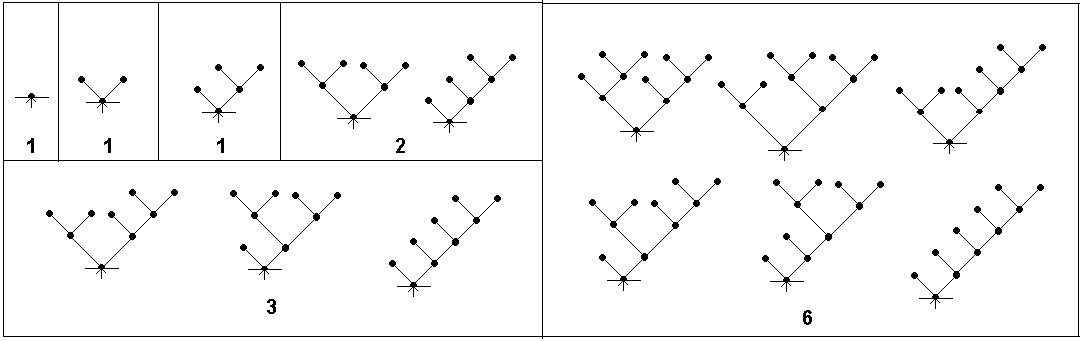
\includegraphics[scale =0.45]{a001190.png}
   %\caption{The isomorphic trees for $n=1,..., 6$ by \url{https://oeis.org/A001190/a001190.gif}.}
 %  \label{fig:isotree}
  % \end{center}
  % \end{figure}
\end{lem}   
                             
\begin{quest}\label{que:hitnum}
For a non-trivial binary tree $T$ and $F(T) \in \Smusati{\delta=1}=\Uclashi{\delta=1}$, is the number of 1-singular variables in $F(T)$ equal $2^{\hts(T)-1}$?
\end{quest}

Some general remarks: 
  \begin{enumerate}
  \item There are exactly two full clause-sets of $\Musati{\delta=1}$, namely $A_0$ and $A_1$.
  \item If a Horn clause-set $F$ (a clause-set with at most one positive literal in each clause) is minimally unsatisfiable, then $F \in \Musati{\delta=1}$.
  \end{enumerate}  
%%%%%%%%%%%%%%%%%%%%%%%%%%%%%%%%%%%%%%%%%%%%%%%
\section{MU(2)}
\label{sec:mu2}

\begin{lem}\label{lem:mu2-mup}
If $F \in \Musati{\delta=2}$ and there is at least one singular variable $v \in \var(F)$, then by an iterated application of singular DP-reduction we get $F' \in \Musatnsi{\delta=2}$.
\end{lem}
\begin{prf}
See Lemma \ref{lem:sDP-infl}.
\end{prf}

\begin{lem}\label{lem:mu2-Fn}
\cite{KleineBuening2000SubclassesMU} If $F \in \Musatnsi{\delta=2}$, then it is in the form of (isomorphism) $\Dt{n}$  for $n \ge 2$ as follows:
  \begin{displaymath}
    \Dt{n} := \set{\set{x_1,\dots,x_n},\set{\ol x_1,\dots,\ol x_n},\set{\ol x_1,x_2}, \dots, \set{\ol x_{n-1},x_n}, \set{\ol x_n,x_1}}.
  \end{displaymath}

\end{lem}
Remarks:
  \begin{enumerate}
  \item According to \cite{KullmannZhao2010Extremal}
  \begin{enumerate}
  \item The only hitting clause-sets amongst the $\Dt{n}$ ($\Uclashnsi{\delta=2}$) are for $n=2,3$. 
  \item All $\Dt{n}$ are saturated, thus $\Musatnsi{\delta=2} = \Smusatnsi{\delta=2}$. Also we have $\minvdeg(\Dt{n}) = 4$. 
  \item $\Dt{n}$ contains two full clauses (one with only positive literals and one with only negative literals) and the rest of clauses are as a cycle $v_1 \ra \dots \ra v_n \ra v_1$ (that at least one variable must be true and one must be false).
  \item By splitting $\Dt{n}$ to $F_0, F_1$ for any variable $v \in \var(\Dt{n})$, we have $F_0, F_1 \in \Musati{\delta=1} $.
  \end{enumerate} 
  \end{enumerate} 
  
\begin{lem}\label{lem:mu2-smu2}
Consider $\Dt{n}$ in Lemma \ref{lem:mu2-Fn}. If we split $\Dt{n}$ to $F_0:=\pao v0 * \Dt{n}$ and $F_1:=\pao v1 * \Dt{n}$ on any variable $v \in \var(\Dt{n})$, then they are not saturated.($F \in \Musatnsi{\delta=2} = \Smusatnsi{\delta=2}$)
\end{lem}
\begin{prf}
Based on Lemma \ref{lem:mu1-sma-uhit}, we have $\Smusati{\delta=1} = \Uclashi{\delta=1}$. Also, since $\Dt{n}$ for $n \ge 4$ is not in $\Uclash$ thus there exists some partial assignment $\vp$ such that $\vp * \Dt{n} \not \in \Musat$. Now, suppose that for all one-variable assignments the result would be in $\Smusati{\delta=1}$. Thus, they would be in $\Uclashi{\delta=1}$, which is stable under partial assignments, and as a result all applications of partial assignments to $\Dt{n}$ would stay in $\Musat$. This yields a contradiction. Since  the literals in $\Dt{n}$ have complete symmetry, thus for $n \ge 4$ no single assignment can yield an element of $\Musati{\delta=1}$.
\end{prf}

\begin{lem}\label{lem:mu2-horn-tree}
Consider splitting $\Dt{n}$ based on Lemma \ref{lem:mu2-smu2} on any variable $v \in \var(\Dt{n})$. Then, $ F_1$ is a Horn clause-set and $ F_0$ is a dual-Horn clause-set. Also, there exist a resolution tree $T$ for $ F_0,F_1$ such that $\hts(T(F_0))= \hts(T(F_1)) \le 1$.
\end{lem}
\begin{prf}
If we split $\Dt{n}$ regarding $x_1$, we have:
\begin{displaymath}
F_0=\set{\set{x_2,\dots,x_n},\set{\ol x_2,x_3},\dots, \set{\ol x_{n-1},x_n},\set{\ol x_n}}.
\end{displaymath}
\begin{displaymath}
F_1=\set{\set{\ol x_2,\dots,\ol x_n},\set{x_2},\set{\ol x_2,x_3}\dots, \set{\ol x_{n-1},x_n}}.
\end{displaymath}
As it can be seen, $F_1$ is a Horn clause-set. Also, if we flip (change the sign) all literals $x$ in  $F_0$ to get $F_0'$, then $F_0'$ is a Horn clause-set and thus, $ F_0$ is a dual-Horn clause-set. Since $\Dt{n}$ have complete symmetry regarding the literals, $F_0, F_1$ for all literals hold these properties. Also, for all Horn clause-sets (and dual-Horn clause-sets) there exist a resolution tree such that $\hts(T) \le 1$.
\end{prf}

\begin{quest}\label{que:mu-2-horn}
If we saturate $F_0, F_1$ in Lemma \ref{lem:mu2-horn-tree}, what would happen to the resolution trees $T(F_0), T(F_1)$ with $\hts(T(F_0))= \hts(T(F_1)) \le 1$?
\end{quest}

\begin{lem}\label{lem:mu2-build}
All $F \in \Musati{\delta=2}$ can be obtained from $\Dt{n}$ (in Lemma \ref{lem:mu2-Fn}) by singular extension of  $\Dt{n}$. Also, for a clause-set $F \in \Musati{\delta=2}$ we can obtain a clause-set $F' \in \Musati{\delta=2}$ via singular extension.
\end{lem}
\begin{prf}
For the first part, consider $F \in \Musati{\delta=2}$. Then, based on Lemma \ref{lem:mu2-Fn} an iterated application of singular DP-reduction leads to $F'=\Dt{n}$. Also, the singular DP-extension is the reverse direction of singular DP-reduction (and does not change the deficiency and minimal unsatisfiability). Thus, we can obtain all $F \in \Musati{\delta=2}$ by singular extension of $\Dt{n}$. For the second part, consider $F \in \Musati{\delta=2}$. Based on definition \ref{def:singularextn}, if $F'$ is obtained by application of singular extension then $F' \in \Musati{\delta=2}$.
\end{prf}
Remarks:
  \begin{enumerate}
  \item There is exactly one full clause-set in $\Musati{\delta=2}$, namely $A_2$ (up to isomorphism).
  \item For $\Dt{n} \in \Smusatnsi{\delta=2}$ and each $v \in \var(\Dt{n})$, $\ve \in \set{0,1}$, holds $\pao v{\ve} * \Dt{n} \in \Musati{\delta=1}$ (by Lemma \ref{lem:smu-mu}).
  \end{enumerate}
  
\begin{lem}\label{lem:mu2-sing}
 By Lemma 5.13 in \cite{KullmannZhao2010Extremal}, if $F \in \Musati{\delta=2}$ with $\minvdeg(F) \ge 4$ then $F$ is singular if and only if $F$ contains a unit-clause.
\end{lem}  

\begin{quest}\label{que:mu-2-ism}
If we extend some of clause-sets in $\Dt{n}$ with different $n$ using Lemma \ref{lem:mu2-build}, is it possible to obtain isomorphic clause-sets with different $n$?
\end{quest}

\begin{quest}\label{que:mu2-from-mu1}
Is every element of $\Musati{\delta=2}$ obtained from some $\Dt{n}$, by expanding every clause via variable-disjoint elements from $\Musati{\delta=1}$ ?
\end{quest}

\begin{quest}\label{que:mu2-uhit2}
How can we describe the subclasses $\Uclashi{\delta=2}$ and $\Smusati{\delta=2}$?
\end{quest}

\begin{quest}\label{que:mu2-hardness}
Based on Section \ref{sec:Hardnessmeasures}, how can we determine the hardness and the width hardness for $F \in \Musati{\delta=2}$? and moreover how can we determine the resolution- and tree-resolution-complexity precisely?
\end{quest}

\begin{quest}\label{que:mu2-count}
Can we count the number of non-isomorphic elements of $F \in \Musati{\delta=2}$ for a given number of clauses?
\end{quest}
%%%%%%%%%%%%%%%%%%%%%%%%%%%%%%%%%%%%%%%%%%%%%%%
\bibliographystyle{plainurl}

\BibliographyOKlibrary



\end{document}

%%% Local Variables: 
%%% mode: latex
%%% TeX-master: t
%%% End: 
